\chapter{Resultados} \label{ch:RD}

No trabalho de Khairunniza-Bejo e Kamarudin (2011), o atributo SST foi previsto em mangas 'Chokanan' a partir do espaço de cores HSV. Os autores construíram modelos de Regressão Linear Simples para cada canal deste espaço de cor, e obtiveram como melhor resultado um coeficiente de correlação igual a -0,92 para o canal Hue. Assim, para as mangas da variedade 'Palmer', também foi construída uma Regressão linear com o atributo Hue como entrada. Entretanto, esperava-se um resultado inferior aos obtidos pelos autores, visto que, para as mangas 'Palmer', o atributo Hue não varia linearmente. A Figura \ref{fig:hue_sst} mostra a variação do SST de acordo com o Hue. 

\begin{figure}[H]
\centering
	\caption{Variação do SST conforme o Hue.}
	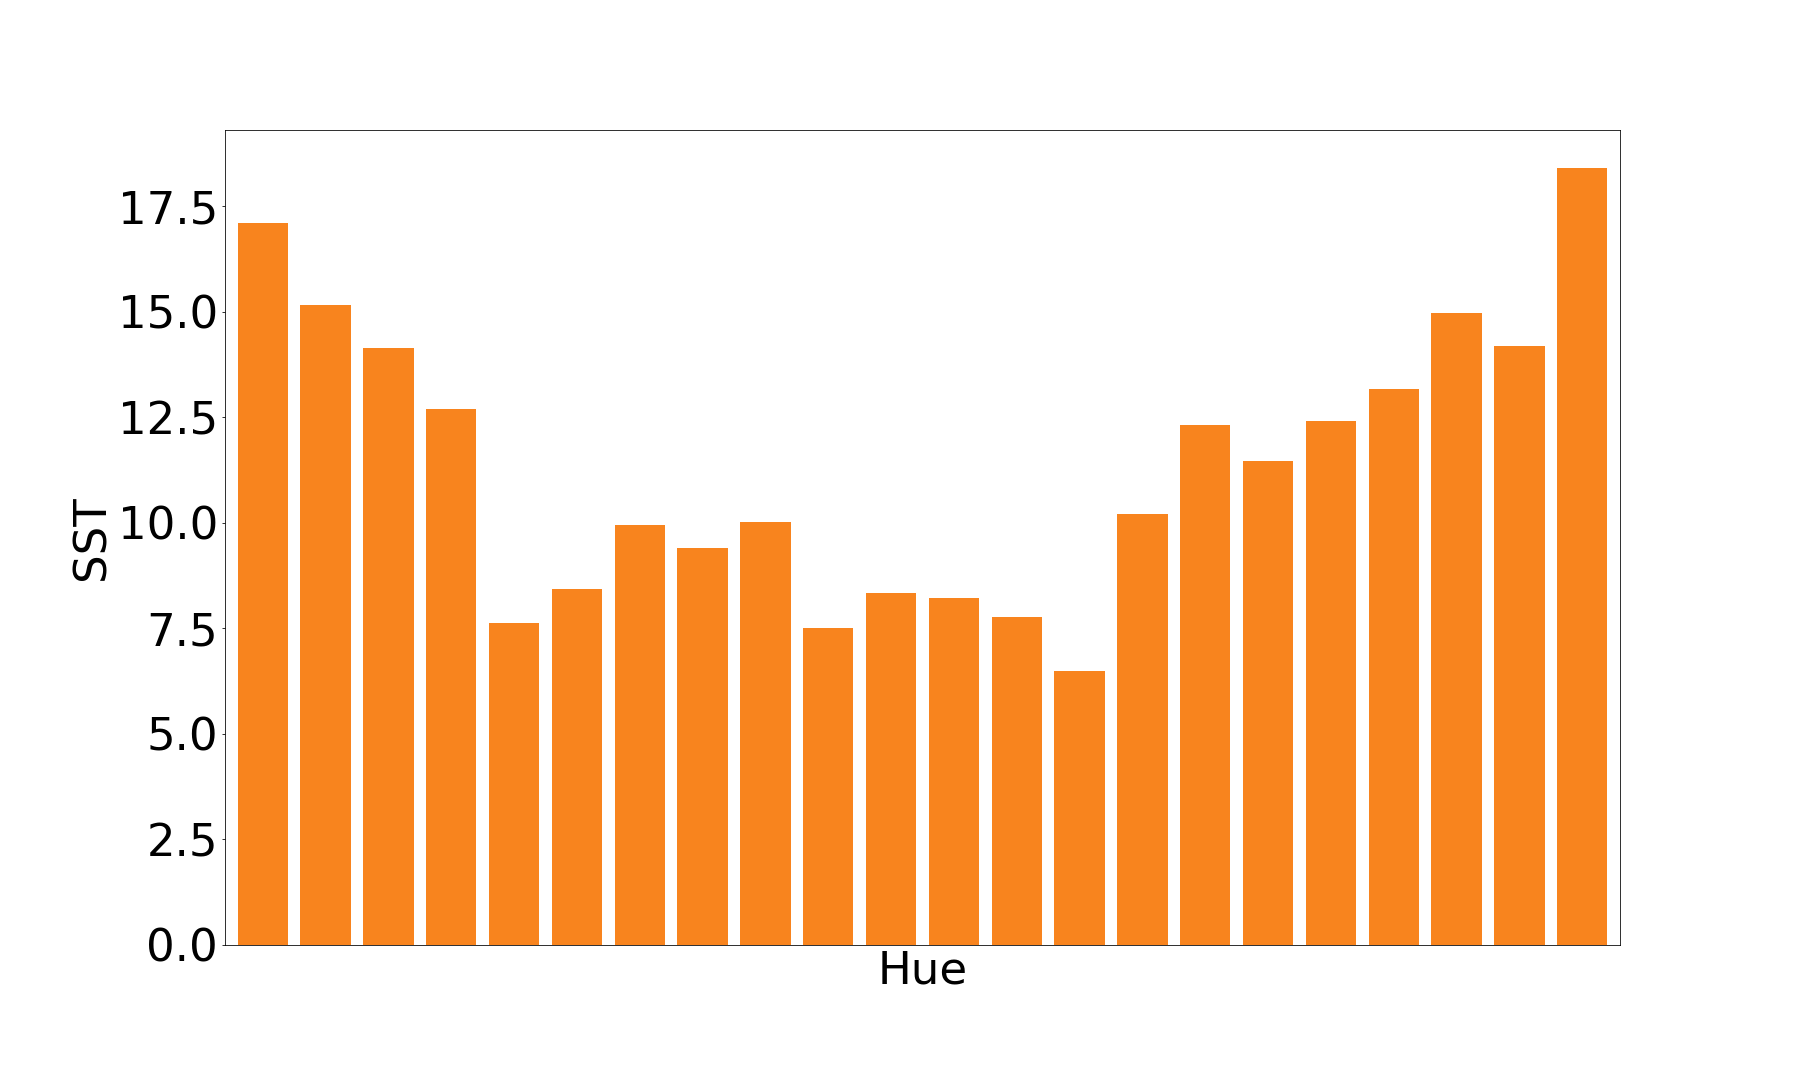
\includegraphics[scale=0.18]{img/hue_sst_palmer.png}
	\legend{\textbf{Fonte:} (Autor, 2019).}\label{fig:hue_sst}
\end{figure}

Conforme esperado, o coeficiente de correlação obtido para a Regressão linear foi muito inferior, com um valor igual a -0,1179. Na Figura \ref{fig:comp_hue} são mostradas a reta ajustada para as amostras do presente estudo e a reta ajustada pelos autores Khairunniza-Bejo e Kamarudin (2011).

\begin{figure}[H]
\centering
    \caption{\label{fig:comp_hue} Modelos de Regressão linear construídos para o atributo Hue (a) Presente estudo (b) Trabalho de Khairunniza-Bejo e Kamarudin (2011).}
    \subcaptionbox{}{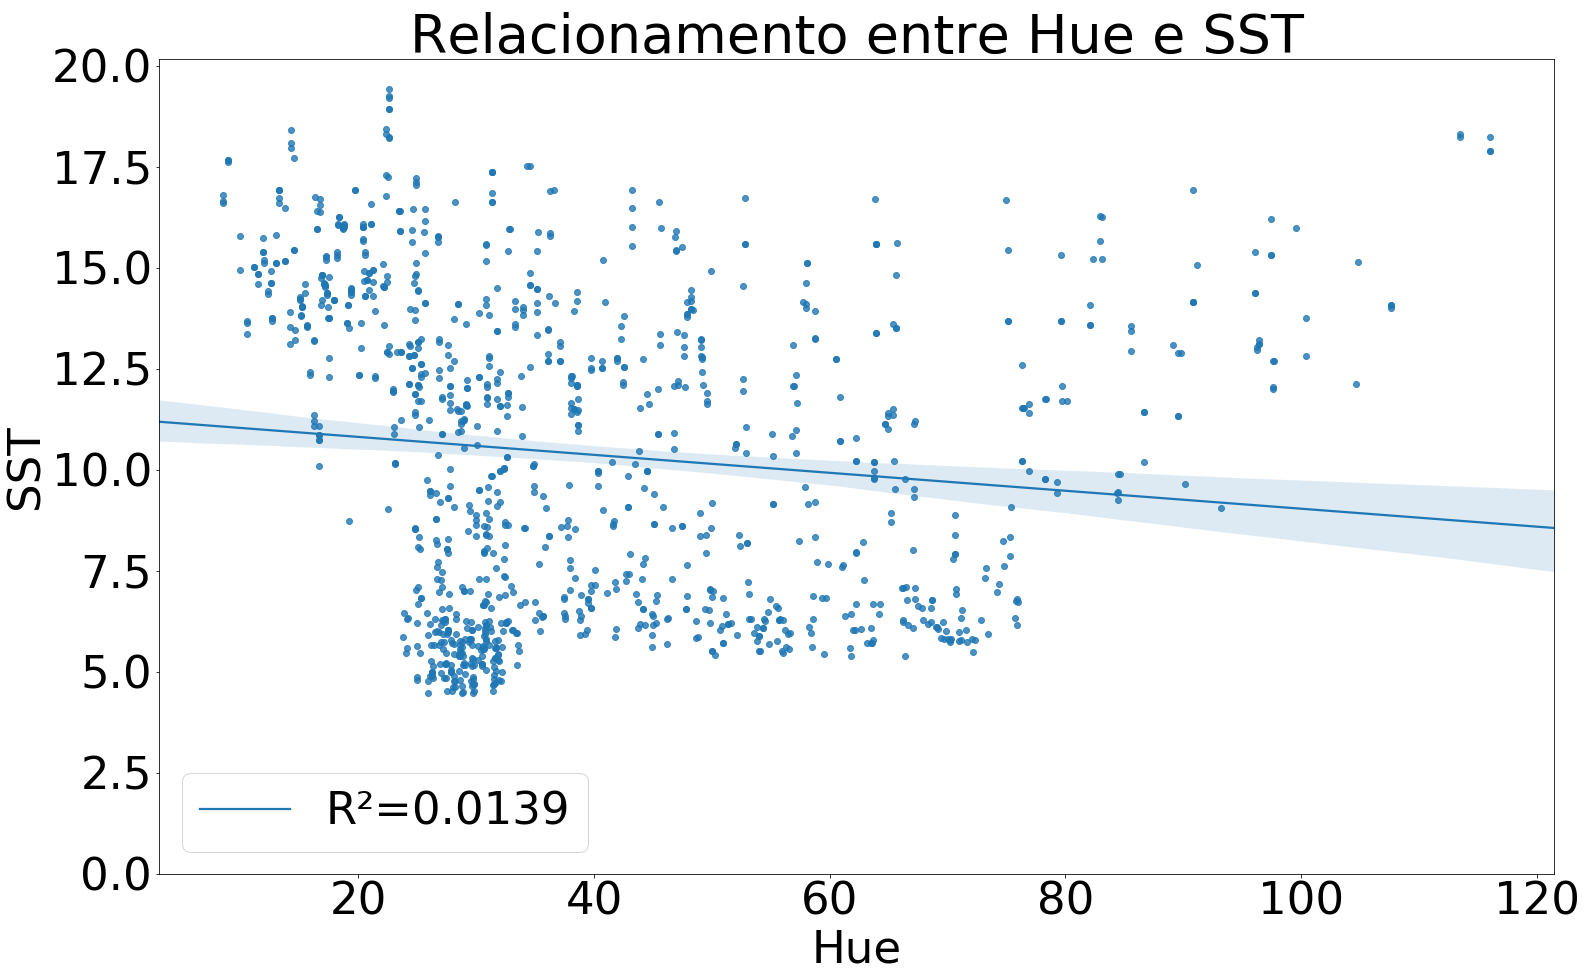
\includegraphics[scale=0.133]{img/scatter_sst_hue_palmer.png}}
    \subcaptionbox{}{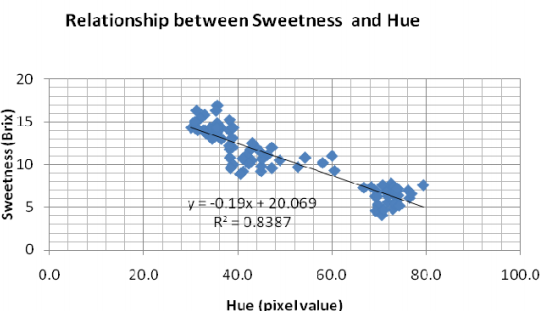
\includegraphics[scale=0.36]{img/sst_lit_hue.png}}
    \legend{\textbf{Fonte: } (Autor, 2019).}
\end{figure}

Devido ao relacionamento não linear entre Hue e SST, esperava-se que com a \textit{Random Forest} fosse obtido um resultado superior. Os valores de $R$ e $RMSE$ obtidos por ela, assim como pela Regressão linear, são mostrados na Figura \ref{fig:fold_sst_hue}, para cada \textit{fold}.

\begin{figure}[H]
\centering
	\caption{Métricas obtidas para cada fold, obtidos para as duas técnicas de inferência (a) Coeficiente de correlação (R) (b) RMSE.}
	\subcaptionbox{}{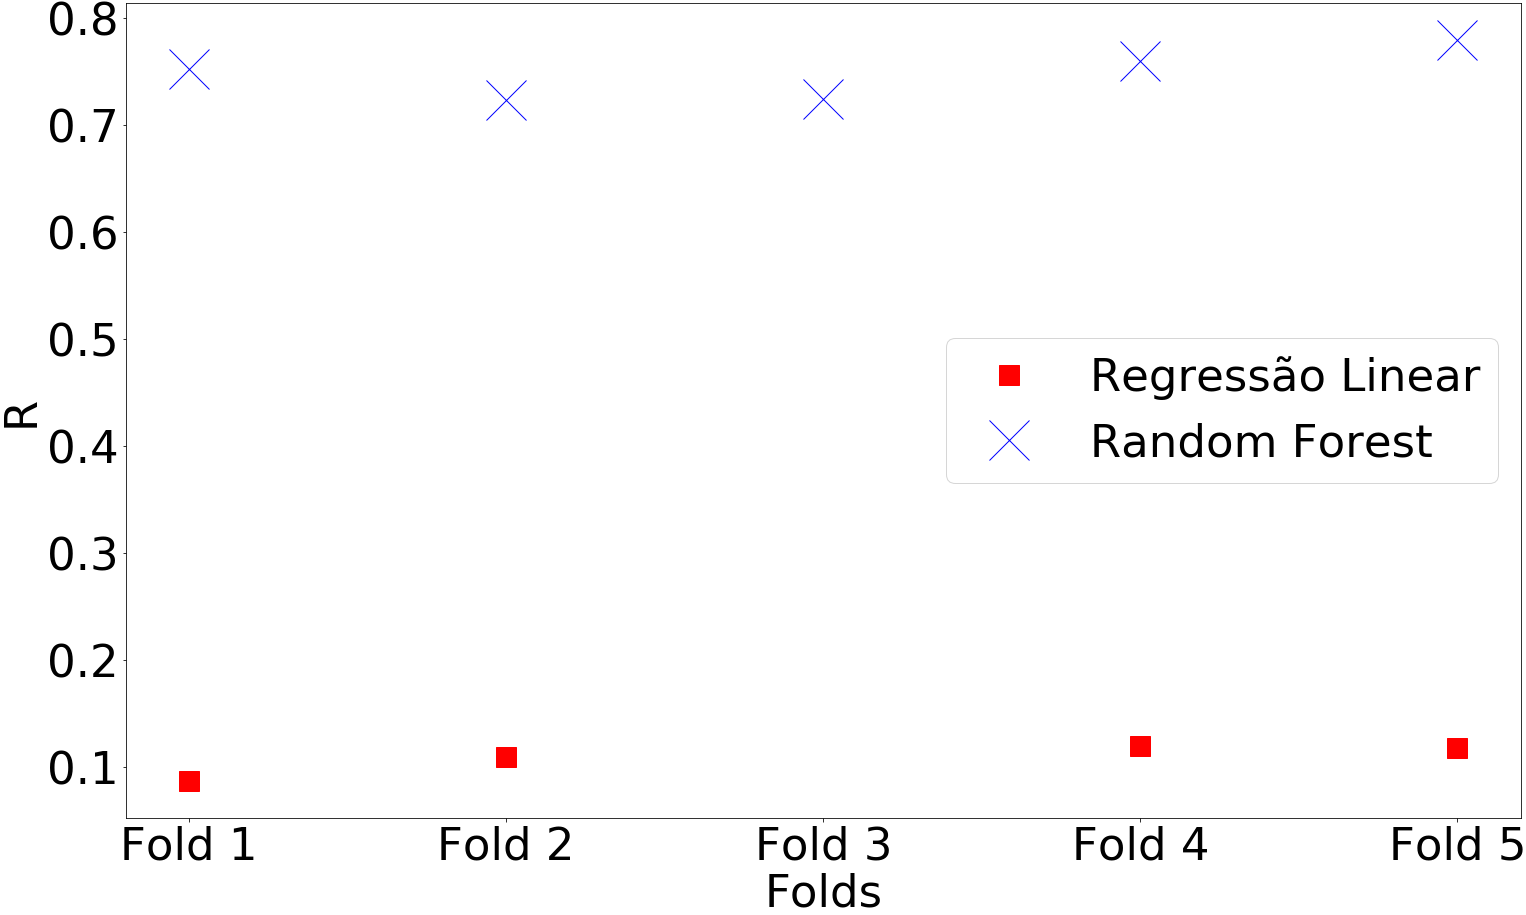
\includegraphics[scale=0.15]{img/fold_r_sst_hue_palmer.png}}
	\subcaptionbox{}{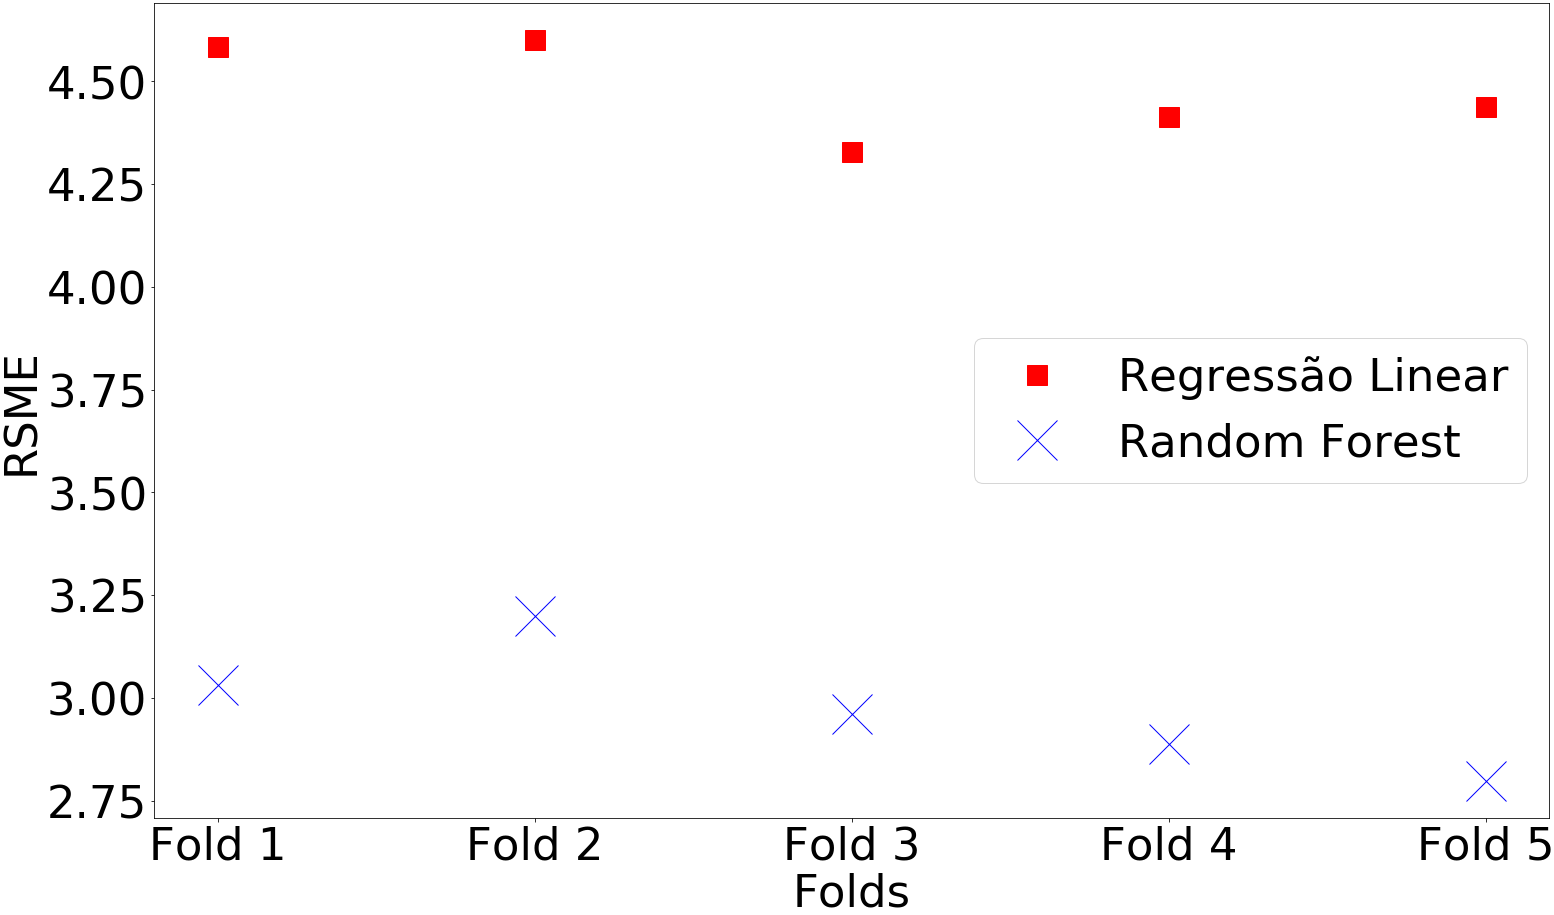
\includegraphics[scale=0.15]{img/fold_rmse_sst_hue_palmer.png}}
	\legend{\textbf{Fonte:} (Autor, 2019).}\label{fig:fold_sst_hue}
\end{figure}

Apesar de a \textit{Random Forest} ser claramente superior, como esperado, o resultado ainda não é razoável. Para as mangas da variedade 'Palmer', vê-se que este atributo não é suficiente para a determinação de SST como foi para as mangas da variedade 'Chokanan'.

Por outro lado, os autores YAHAYA et al. (2015) testaram o espaço de cores RGB e obtiveram um coeficiente de correlação igual a 0,814 e RMSE igual a 1,218 ªBrix. Para verificar se existe uma relação linear entre as variáveis RGB extraídas das mangas 'Palmer' e o SST, foram plotadas as variações das mesmas, mostradas na Figura \ref{fig:rgb_sst}.

\begin{figure}[H]
\centering
    \caption{\label{fig:rgb_sst} Variação das variáveis RGB para o SST (a) Canal R (b) Canal G (c) Canal B.}
    \subcaptionbox{}{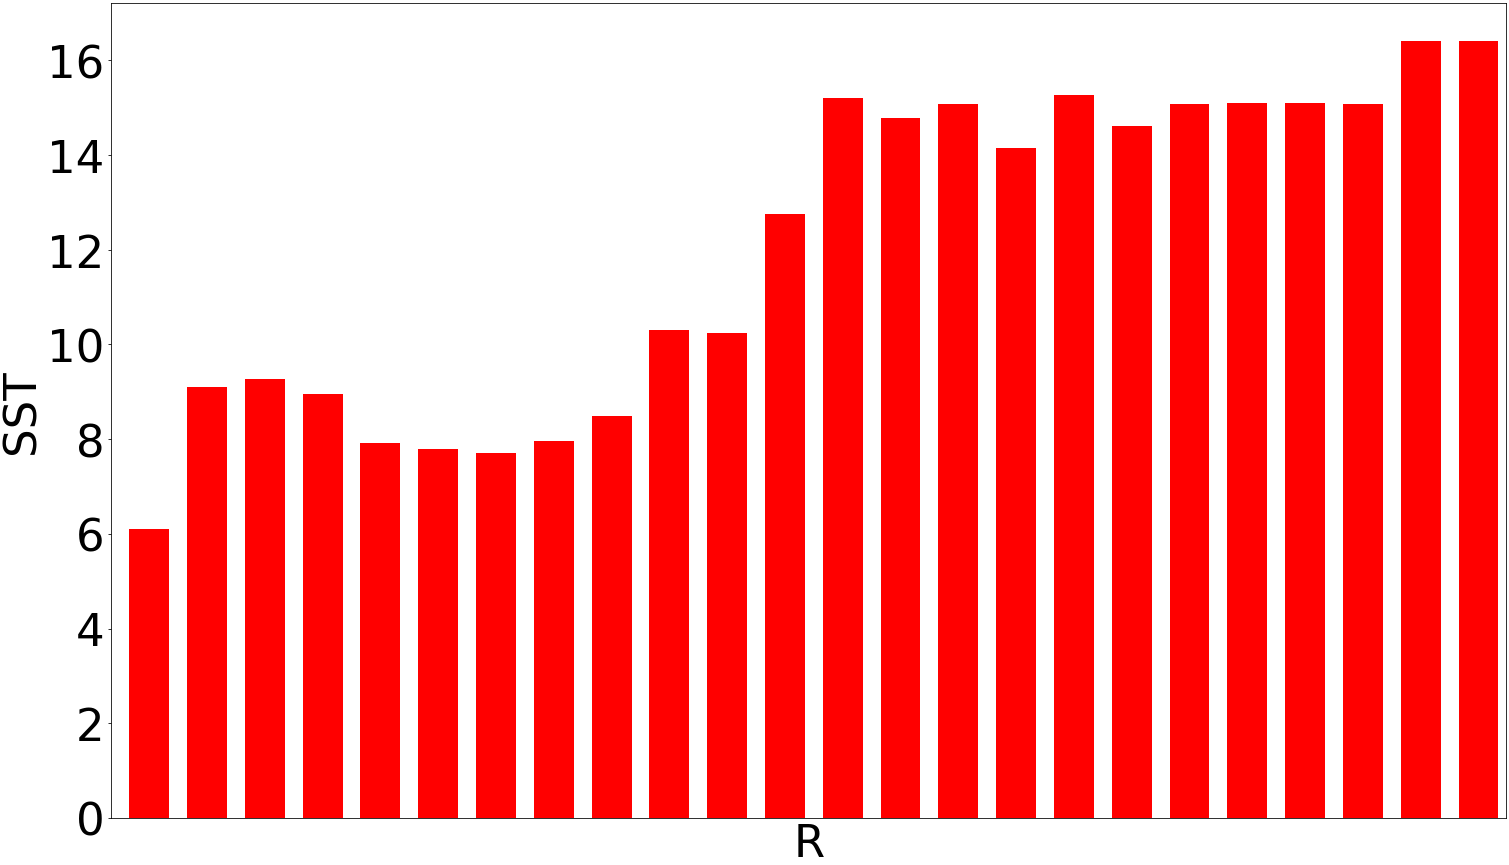
\includegraphics[scale=0.12]{img/R_sst_palmer.png}}
    \subcaptionbox{}{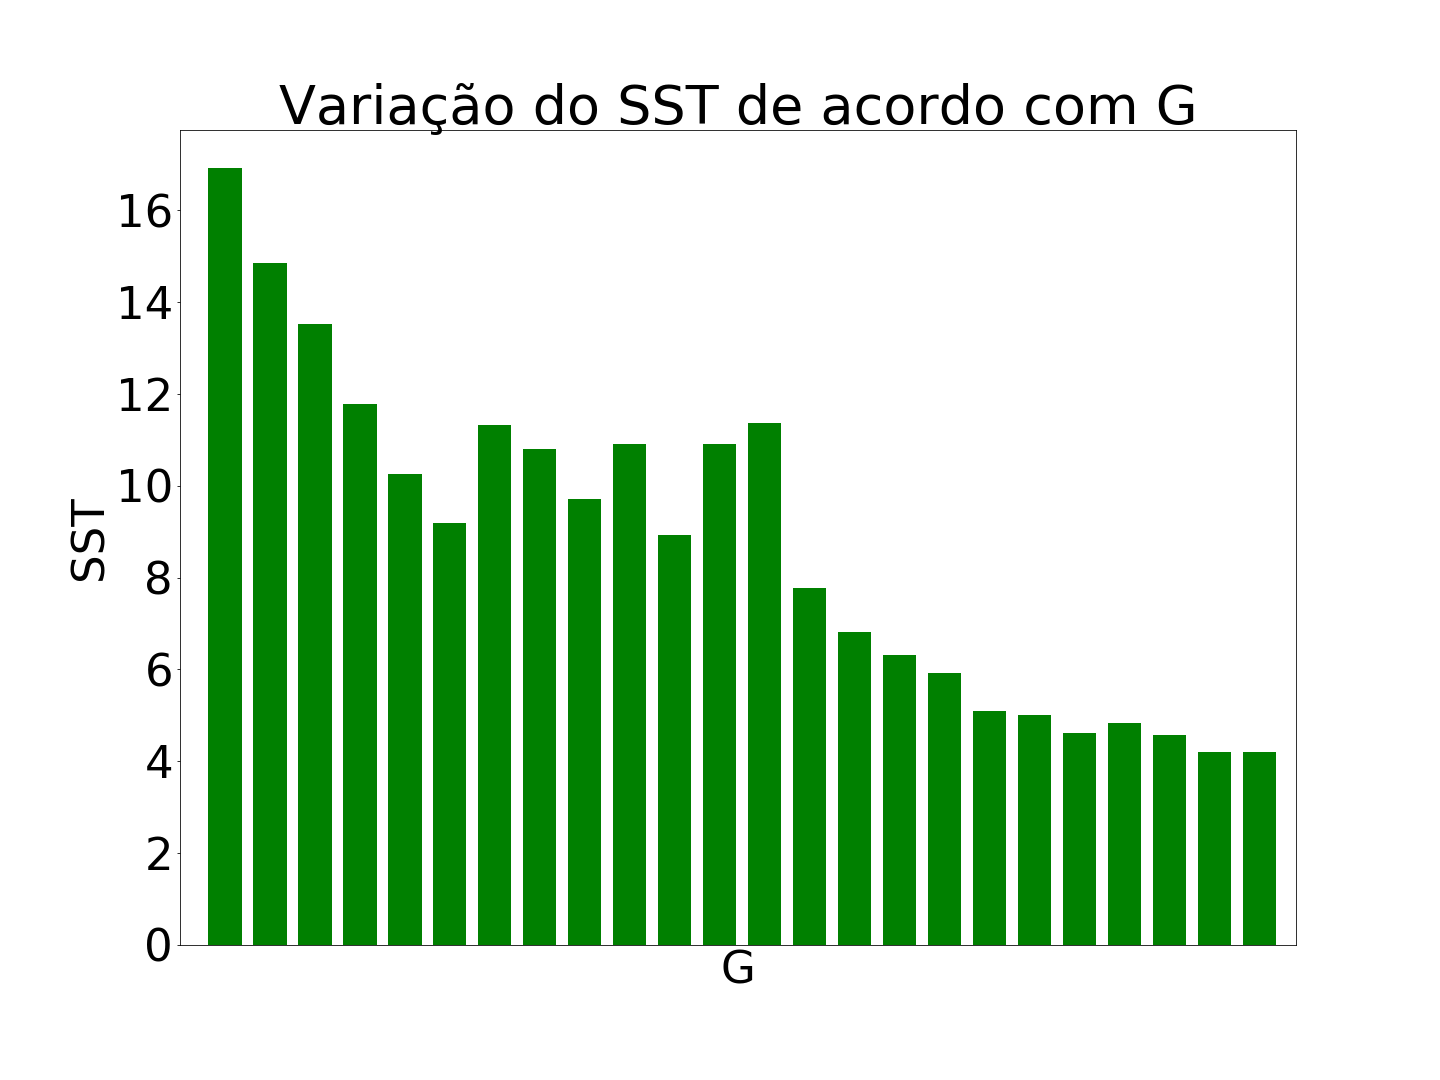
\includegraphics[scale=0.12]{img/G_sst_palmer.png}}
    \subcaptionbox{}{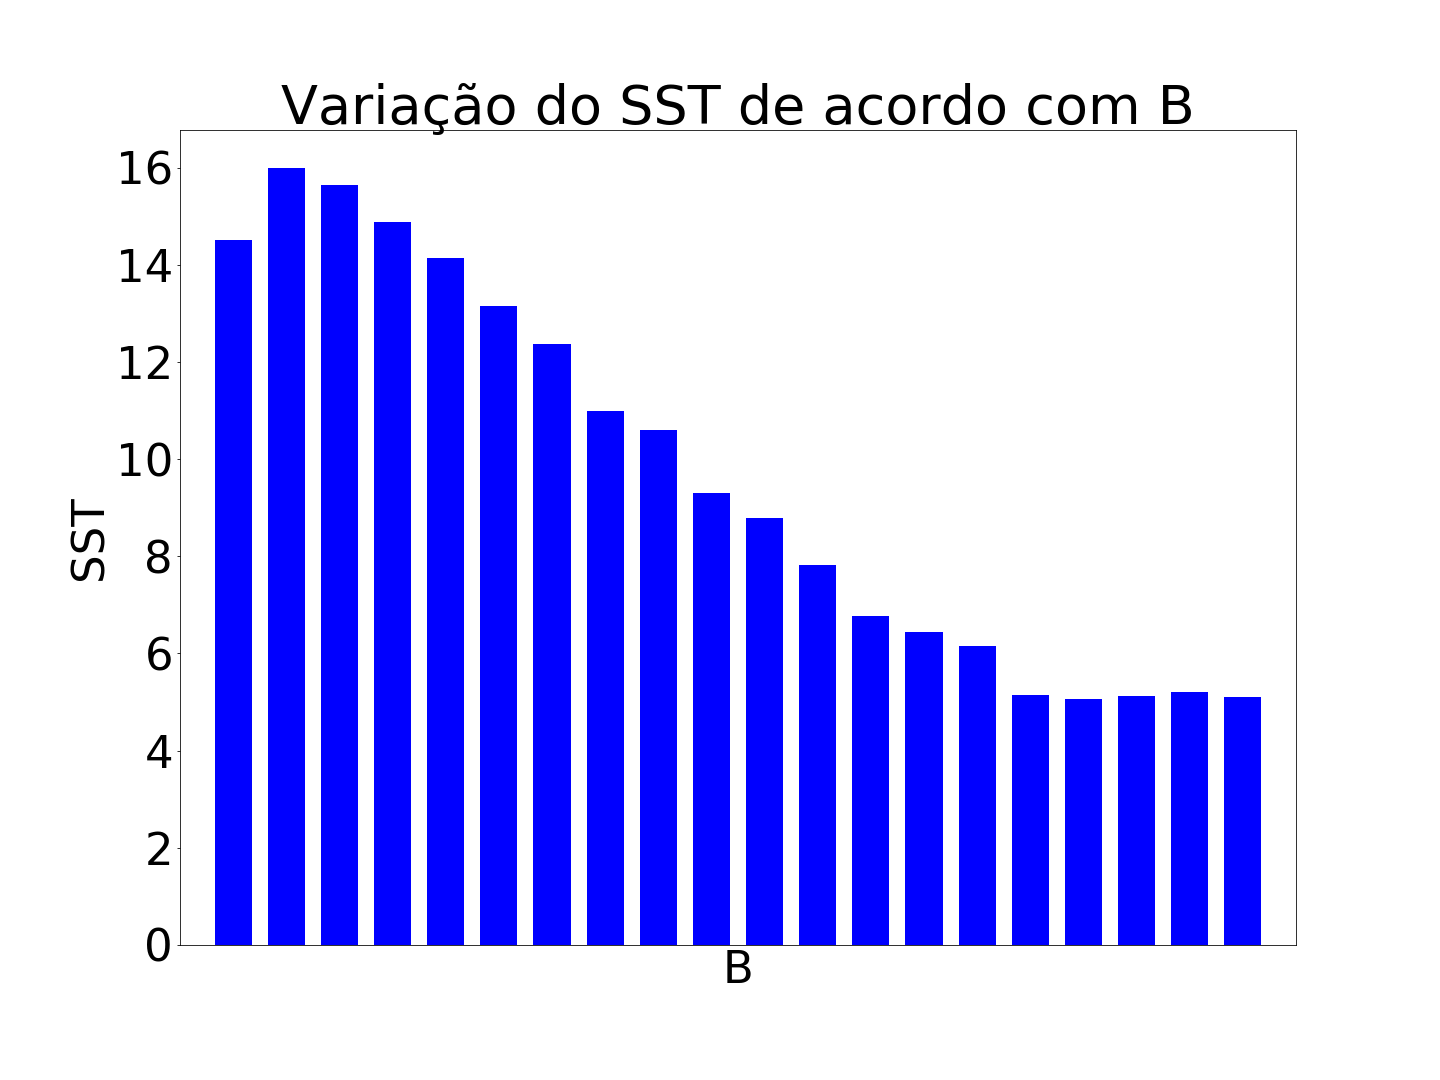
\includegraphics[scale=0.12]{img/B_sst_palmer.png}}
    \legend{\textbf{Fonte: } (Autor, 2019).}
\end{figure}

Nota-se uma variação aproximadamente linear para as três variáveis. Assim, espera-se um resultado razoável para a Regressão Linear Múltipla. Na figura \ref{fig:fold_sst_rgb} são mostrados os valores de R e RMSE para a Regressão Linear e \textit{Random Forest} em todos os \textit{folds}.

\begin{figure}[H]
\centering
	\caption{Métricas obtidas para cada fold, obtidos para as duas técnicas de inferência (a) Coeficiente de correlação (R) (b) RMSE.}
	\subcaptionbox{}{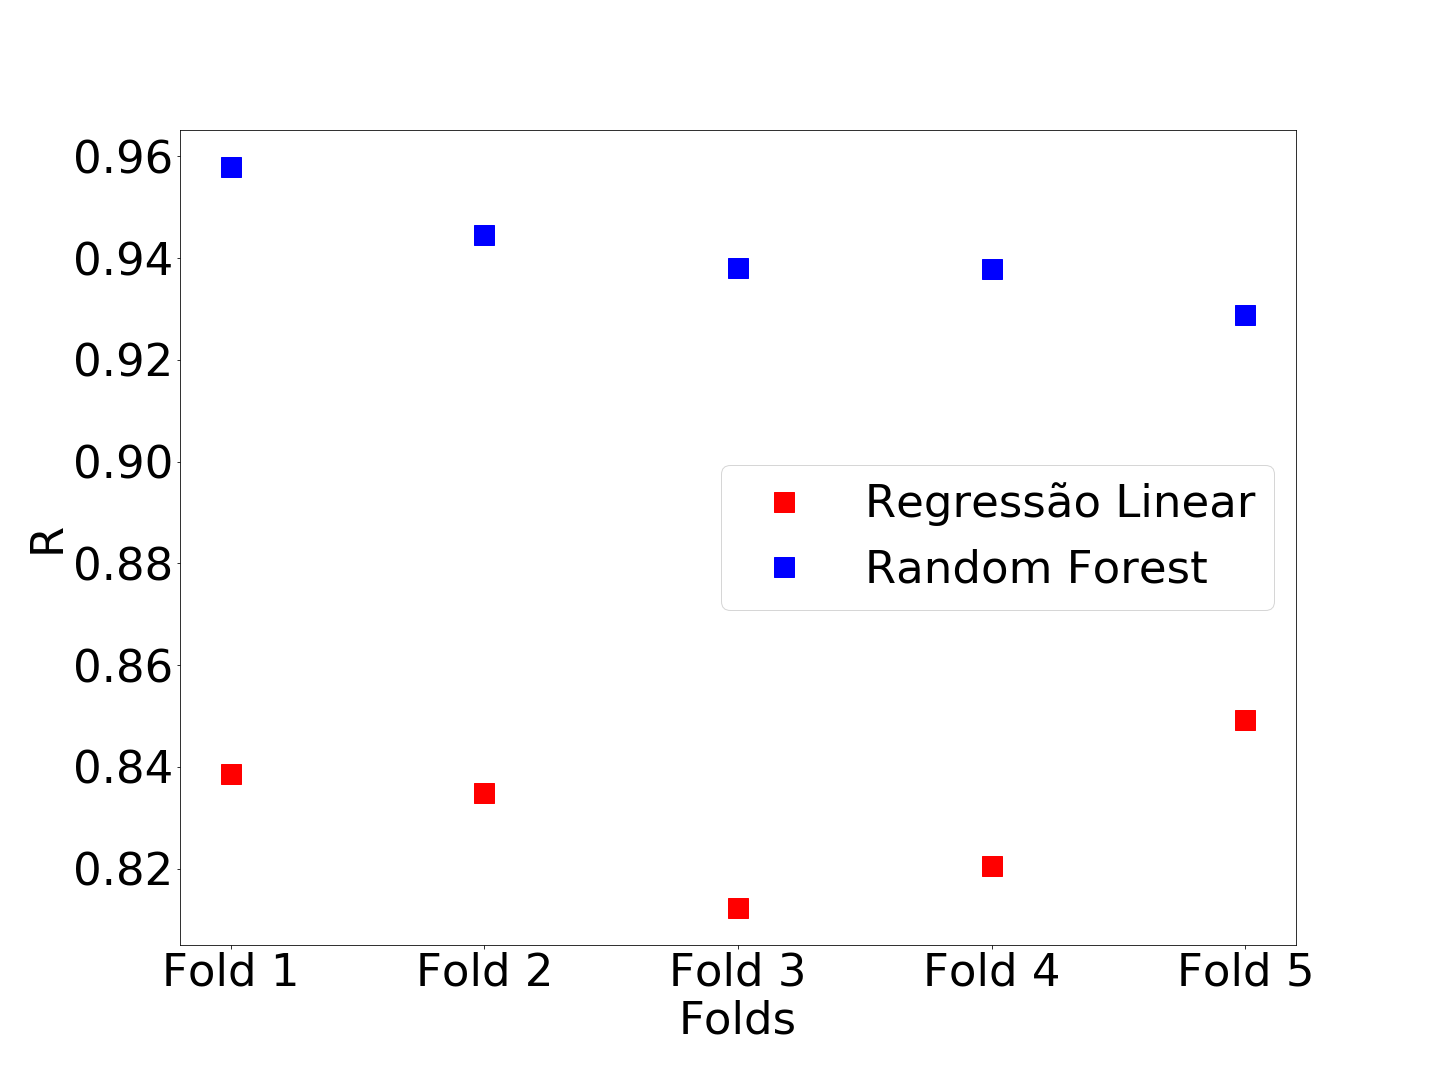
\includegraphics[scale=0.15]{img/fold_r_sst_rgb_palmer.png}}
	\subcaptionbox{}{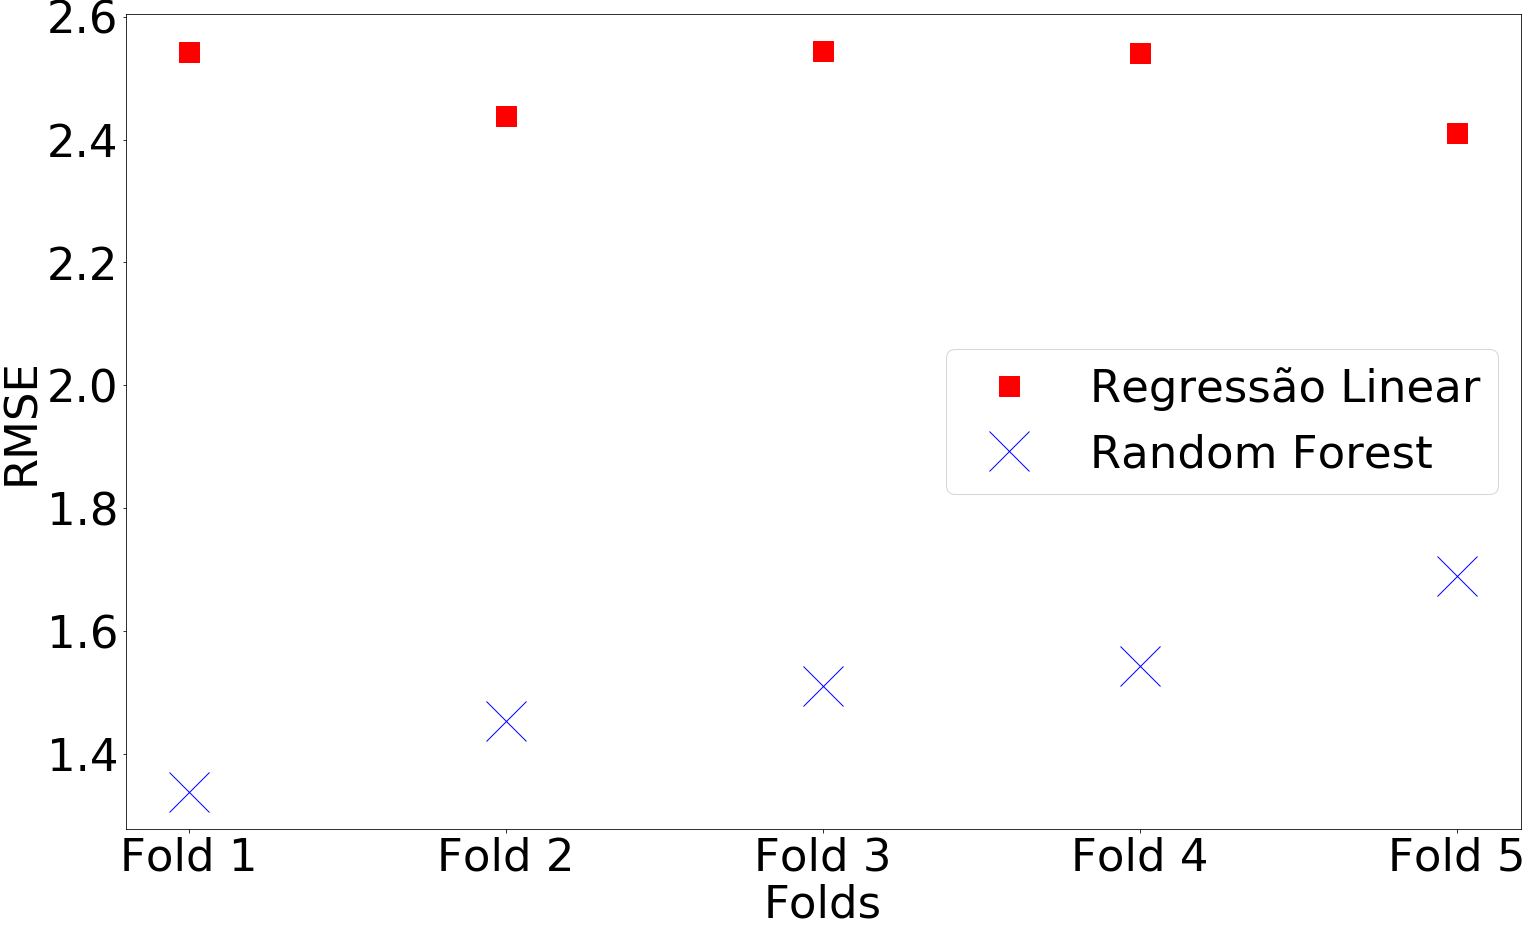
\includegraphics[scale=0.15]{img/fold_rmse_sst_rgb_palmer.png}}
	\legend{\textbf{Fonte:} (Autor, 2019).}\label{fig:fold_sst_rgb}
\end{figure}

Os valores médios dos coeficientes de correlação para a MLR e RF foram, respectivamente, iguais a 0,8312 e 0,9415. Ambos modelos mostraram-se superiores ao modelo construído por YAHAYA et al. (2015). Entretanto, o valor de RMSE obtido por eles ainda mostra-se menor que os alcançados para as mangas 'Palmer'. 

Desta forma, para a obtenção de um modelo que seja melhor que os da literatura em todas as métricas, foi treinada uma \textit{Random Forest} com todas as variáveis listadas na Tabela \ref{tbl:var_gps}. Com um maior número de variáveis de entrada, há uma maior quantidade de informações associada à cada manga, aumentando-se assim a probabilidade de alcançar melhores resultados. Os valores de R e RMSE para cada \textit{fold} do modelo RF com todas as variáveis são mostrados na Tabela \ref{tbl:r_rmse_all}.

\begin{table}[H]
	\centering
	\caption{\label{tbl:r_rmse_all} Valores de R e RMSE obtidos para o modelo \textit{Random Forest} com todas as variáveis.}
	\begin{tabular}{lll}
	\hline
	Fold  & R      & RMSE   \\ \hline
	1     & 0,9723 & 1,0018 \\ \hline
	2     & 0,9405 & 1,0987 \\ \hline
	3     & 0,9755 & 0,7075 \\ \hline
	4     & 0,9634 & 0,9029 \\ \hline
	5     & 0,9660 & 0,8104 \\ \hline
	Média & 0,9789 & 0,9042	\\ \hline
	\end{tabular}
	\legend{\textbf{Fonte: } (Autor, 2019).}
\end{table}

O coeficiente de correlação obtido foi maior que o encontrado pelos autores Khairunniza-Bejo e Kamarudin (2011) e YAHAYA et al. (2015), assim como o valor de RMSE foi menor que o obtido por estes.

% \section{Seção de exemplo 1 - Códigos} \label{sec:resex1}

% \subsection{Subseção de exemplo 1 - Inserindo trechos de códigos}
 
% O nosso querido Leonardo Cavalcante providenciou um comando que deixa nossos trechos de códigos bonitinhos e gera um elemento pré-textual de Lista de Códigos. 

% Os códigos são adicionados através do comando seguinte:

% \textbackslash sourcecode\{ Descrição \}\{Label\}\{Linguagem\}\{Arquivo com extensão\}

% Um exemplo pode ser visto no código \ref{cmd:cron} abaixo.

% \sourcecode{Configuração do intervalo de execução no Script Agendador}{cron}{javascript}{cron.js}


% \section{Seção de exemplo 2 - Listas} \label{sec:resex2}

% \subsection{Subseção de exemplo 2 - Lista de itens} 

% Existem alguns tipos de listas no Latex, iremos exemplificar a lista sem numeração (seção \ref{subsubsec:itemize}), a lista enumerada (seção \ref{subsubsec:enumerate}) e a lista mista (seção \ref{subsubsec:mista}). As listas podem ser encadeadas de diversas maneiras,
% de acordo com a necessidade do autor.

% \subsubsection{Subsubseção de exemplo 1 - Lista sem numeração} \label{subsubsec:itemize}

% Este é um exemplo de lista sem numeração.

% \begin{itemize}
% 	\item \textbf{Cadastrar usuário}

% 		\begin{itemize}
%     		\item Atores
% 		    	\begin{itemize}
%     		    	\item Usuário
% 		    	\end{itemize}

% 	    	\item Fluxo de eventos primário
% 			    \begin{itemize}
% 	    		    \item o usuário deve se cadastrar informando seu nome, \textit{e-mail} e senha;
% 		        	\item a API armazena os dados do usuário;
% 		    	    \item o usuário é liberado para realizar o \textit{login}.
% 			    \end{itemize}

%     		\item Fluxo alternativo
% 			    \begin{itemize}
% 		    	   \item o usuário desiste de se cadastrar e cancela o caso de uso clicando no botão voltar.
% 	    		\end{itemize}

% 		\end{itemize}
	
% \end{itemize}

% \subsubsection{Subsubseção de exemplo 2 - Lista enumerada} \label{subsubsec:enumerate}

% Este é um exemplo de lista enumerada.

% \begin{enumerate}
% 	\item O Usuário deseja ver o histórico das variáveis climáticas, então através da interface de usuário escolhe o período ao qual o histórico se refere;
% 	\item A aplicação solicita à API através de uma requisição HTTP contendo o momento de início e o momento do fim do período em seus parâmetros;     			\item A API recebe a solicitação e se comunica com a base de dados, então requere as informações quem possuem a data de leitura no intervalo escolhido;
% 	\item A base de dados retorna os dados em formato Json para a API;
% 	\item A API responde à requisição retornando os dados, também em formato Json, para a aplicação cliente;
% 	\item A aplicação cliente renderiza os gráficos utilizando o conjunto de dados obtidos.
% \end{enumerate}

% \subsubsection{Subsubseção de exemplo 3 - Lista mista} \label{subsubsec:mista}

% Este é um exemplo de lista mista.

% \begin{itemize}
% 	\item \textbf{Cadastrar usuário}

% 		\begin{itemize}
%     		\item Atores
% 		    	\begin{itemize}
%     		    	\item Usuário
% 		    	\end{itemize}

% 	    	\item Fluxo de eventos primário
% 			    \begin{enumerate}
% 	    		    \item o usuário deve se cadastrar informando seu nome, \textit{e-mail} e senha;
% 		        	\item a API armazena os dados do usuário;
% 		    	    \item o usuário é liberado para realizar o \textit{login}.
% 			    \end{enumerate}

%     		\item Fluxo alternativo
% 			    \begin{itemize}
% 		    	   \item o usuário desiste de se cadastrar e cancela o caso de uso clicando no botão voltar.
% 	    		\end{itemize}

% 		\end{itemize}

% 	\item \textbf{Visualizar dados atuais}

% 		\begin{itemize}
% 		    \item Atores
% 	    		\begin{itemize}
% 		    	    \item Usuário
% 			    \end{itemize}
    
% 	    	\item Pré-condições
% 			    \begin{itemize}
% 		     	   \item o usuário deve estar autenticado
% 			    \end{itemize}

% 	    	\item Fluxo de eventos primário
% 			    \begin{enumerate}
% 		    	    \item o usuário deve efetuar o \textit{login} informando o \textit{e-mail} e a senha;
% 	    		    \item caso o usuário não seja autenticado, o sistema informa a respeito de credenciais inválidas e encerra o caso de uso;
% 		    	    \item a API autentica o usuário;
%     			    \item o usuário é liberado para visualizar os dados atuais dos sensores da estação;
% 		        	\item após a visualização o usuário pode finalizar o caso de uso ou efetuar uma nova consulta se desejar.
% 			    \end{enumerate}

%     		\item Fluxo alternativo
% 			    \begin{itemize}
%     			   \item o usuário desiste de visualizar os dados atuais e cancela o caso de uso clicando no botão voltar.
% 			    \end{itemize}

% 		\end{itemize}

% 	\item \textbf{Visualizar histórico}

% 		\begin{itemize}
% 		    \item Atores
% 	    		\begin{itemize}
% 		    	    \item Usuário
% 	    		\end{itemize}

% 	    	\item Pré-condições
%     			\begin{itemize}
% 			        \item o usuário deve estar autenticado
% 			    \end{itemize}

% 		    \item Fluxo de eventos primário
% 			    \begin{enumerate}
% 			        \item o usuário deve efetuar o \textit{login} informando o \textit{e-mail} e a senha;
% 			        \item caso o usuário não seja autenticado, o sistema informa a respeito de credenciais inválidas e encerra o caso de uso;
% 			        \item a API autentica o usuário;
% 			        \item o usuário é liberado para escolher qual período cujo histórico será exibido;
% 			        \item o usuário seleciona as variáveis a serem exibidas no gráficos de linhas;
% 			        \item após a visualização do histórico o usuário pode finalizar o caso de uso se desejar.
% 			    \end{enumerate}

% 		    \item Fluxo alternativo
% 			    \begin{enumerate}
% 			        \item após a escolha do período de exibição do histórico o usuário pode voltar para a tela anterior e escolher um novo período;
% 			        \item o histórico é exibido para o usuário;
% 			        \item após a visualização do histórico o usuário pode finalizar o caso de uso ou efetuar uma nova consulta se desejar.
% 			    \end{enumerate}

% 		    \item Fluxo alternativo
% 			    \begin{enumerate}
% 			        \item o usuário desiste de visualizar o histórico e cancela o caso de uso clicando no botão voltar.
% 			    \end{enumerate}
% 		\end{itemize}
% \end{itemize}